%\section{Results}
%Here results will be presented, with numbers and maybe some graphs or plots of the numbers.


The outcome measures calculated for each subject can be seen in \tabref{tab:measures}.

\begin{table}[h]
	\begin{tabular}{|l|l|l|l|}
		\hline
		& Novice            & Intermediate      & Master            \\ \hline
		Length    & $0.253 \pm 0.043$ & $0.293 \pm 0.004$ & $0.303 \pm 0.040$ \\ \hline
		Span      & $0.407 \pm 0.008$ & $0.415 \pm 0.012$ & $0.433 \pm 0.045$ \\ \hline
		Frequency & $0.071 \pm 0.043$ & $0.062 \pm 0.022$ & $0.121 \pm 0.014$ \\ \hline
		Intensity & $0.758 \pm 0.013$ & $0.775 \pm 0.003$ & $0.783 \pm 0.003$ \\ \hline
	\end{tabular}
	\caption{Outcome measures for each subject. Average measurement found over the three repetitions each subject performed.}
	\label{tab:measures}
\end{table}

The final performance score for each subject is presented in \tabref{tab:scores}.

\begin{table}[h]
	\begin{tabular}{|l|l|l|l|}
		\hline
				          & Novice                     & Intermediate           & Master                   \\  \hline
		Avg. Score & 9.532 $\pm$ 0.292 & 8.579 $\pm$ 0.101 & 7.278 $\pm$ 0.891 \\ \hline
	\end{tabular}
\caption{Performance scores for each subject}
\label{tab:scores}
\end{table}

A Kruskal-Wallis test has been implemented for the statistical analysis of the scores and intensity measure, as the data comes from non-Gaussian distributed data, and the comparison is between three unmatched groups. The other measures were from a Gaussian distribution according to a Kolmogorov-Smirnov test, and a one-way ANOVA was implemented for these. The results from the statistical tests were analysed using Bonferroni correction to compensate for the comparison of three groups, and avoid false negatives or positives. The results of the statistical analysis are presented in \tabref{tab:pValues}.

\begin{table}[h]
	\begin{tabular}{|l|l|l|l|l|}
		\hline
		& Overall & N vs. I & N vs. M & I vs. M \\ \hline
		Length:    & 0.243   & 0.382   & 0.249   & 0.933   \\ \hline
		Span:      & 0.316   & 0.936   & 0.318   & 0.472   \\ \hline
		Frequency: & 0.095   & 0.925   & 0.170   & 0.105   \\ \hline
		Intensity: & 0.039   & 0.549   & 0.030   & 0.295   \\ \hline
		Score:     & 0.027   & 0.372   & 0.020   & 0.372   \\ \hline
	\end{tabular}
	\caption{Statistical analysis p-values for comparison between subjects}
	\label{tab:pValues}
\end{table}


\begin{figure}[H]
	\hfill
	{%
		\begin{minipage}{0.46\linewidth}
			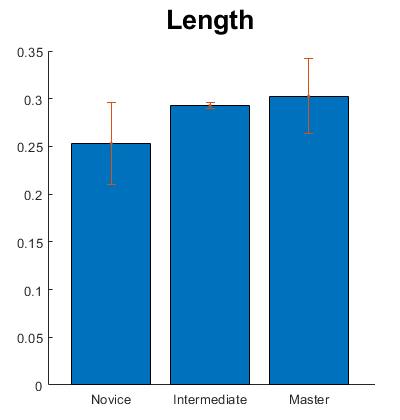
\includegraphics[width=\linewidth]{figures/Length}
			\caption{leave blank}
			\label{fig:Length}
		\end{minipage}
	}\hfill
	{%
		\begin{minipage}{0.46\linewidth}
			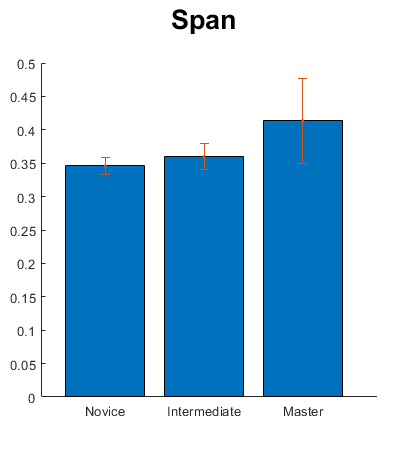
\includegraphics[width=\linewidth]{figures/Span}
			\caption{leave black}
			\label{fig:Span}
		\end{minipage}
	}%\hfill\strut
	\caption{Barcharts of the lenght and span measures. No significant differences were found between subjects in either measure.}
\end{figure}

\begin{figure}[H]
	\hfill
	{%
		\begin{minipage}{0.46\linewidth}
			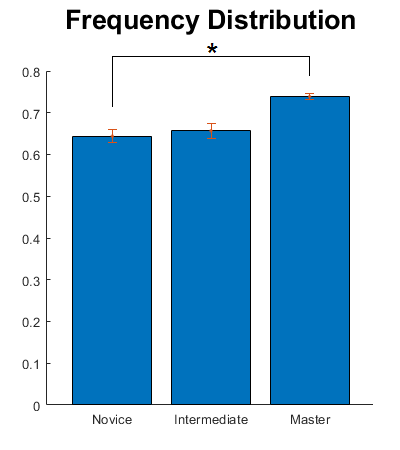
\includegraphics[width=\linewidth]{figures/Distribution}
			\caption{leave blank}
			\label{fig:VelocityChange}
		\end{minipage}
	}\hfill
	{%
		\begin{minipage}{0.46\linewidth}
			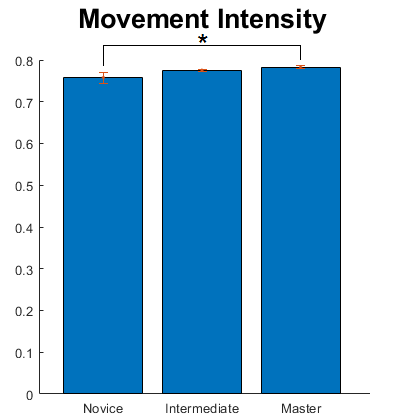
\includegraphics[width=\linewidth]{figures/Intensity}
			\caption{leave black}
			\label{fig:MovementIntensity}
		\end{minipage}
	}%\hfill\strut
	\caption{Barcharts of the velocity change and movement intensity measures. No significant differences were found between subjects in the velocity change measure. Significant difference was found between the novice and master subjects for the movement intensity measure.}
\end{figure}

\begin{figure}[H]
	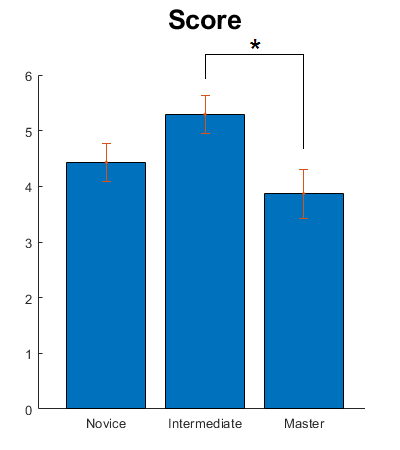
\includegraphics[width=.5\textwidth]{figures/Score}
	\caption{Barchart of the score between subjects. Significant difference was found between the novice and master subjects.}
	\label{fig:Score}  %<--remember LABEL!
\end{figure}


No significant difference was found within either of the length, span or velocity change measures. The intensity measure showed a significant difference ($p<0.05$) between the novice ($0.758 \pm 0.013$) and the master ($0.783 \pm 0.003$).

The analysis of the scores showed a significant difference ($p<0.05$) between the novice ($9.532 \pm 0.292$) and the master ($7.278 \pm 0.891$). Otherwise no difference was to be found within the scores.
